\chapter{REVISÃO DA LITERATURA}\label{chp:REVISAO}

Parte principal do trabalho, que contém a exposição ordenada e pormenorizada do assunto. É composta de revisão de literatura, dividida em seções e subseções, material e métodos e/ou metodologia e resultados, agora descritos detalhadamente. Cada seção ou subseção deverá ter um título apropriado ao conteúdo.
Deve-se utilizar sempre a terceira pessoa do singular na elaboração do texto, mantendo-se a forma impessoal

\section{Intruções para uso do documento}

De modo a facilitar a construção do texto, abaixo serão explicados os elementos necessários para a construção do texto:

\subsection{Negrito e Italico}
Colocar um texto em \textit{italico}, \textbf{negrito}.

\subsection{Listas numeradas}
Nesta lista numerada, com alguns exemplos de citação:
\begin{enumerate}
    \item Esta é uma citação ao final da linha \cite{Pressman2011},
    \item De acordo com \textcite{Pressman2011}, está é uma citação no meio da linha.
    \item Este é um exemplo de nota de rodapé do site da UTFPR\footnote{https://www.utfpr.edu.br/}
\end{enumerate}

\subsection{Listas não numeradas}
Este é um exemplo de lista não numerada:
\begin{itemize}
    \item Primeiro item da lista;
    \item Segundo item da lista;
    \item Terceiro item da lista;
\end{itemize}

\subsection{Figuras}
Na Figura \ref{fig:label-uma-figura}, temos um exemplo de figura, onde a largura dela é definida com base na largura da página (columnwidth) e com autoria própria.

\begin{figure}[htb]
	\centering
	\caption{Um exemplo de figura}
	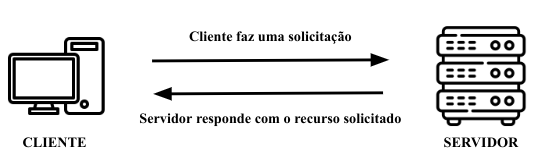
\includegraphics[width = 0.8\columnwidth]{../Images/cliente-servidor.png} 
	\newline \footnotesize \textbf{Fonte: Autoria própria (2024).}
	\label{fig:label-uma-figura}
\end{figure}

Aqui, Figura \ref{fig:outra-figura}, temos um exemplo de figura, onde a largura dela é definida com base na largura da página (columnwidth) e adaptada de uma referencia qualquer.

\begin{figure}[htb]
	\centering
	\caption{Outro exemplo de figura}
	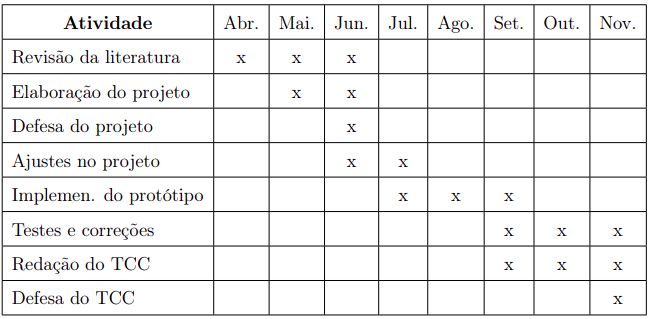
\includegraphics[width = \columnwidth]{../Images/cronograma.png} 
	\newline \footnotesize \textbf{Fonte: Adaptada de \textcite{Pressman2011, Capes2018}}
	\label{fig:outra-figura}
\end{figure}

\subsection{Tabelas}
Para elementos tabulares, deve-se usar o modelo da Tabela \ref{tab:tabela-dados}. Também é possível adicionar notas à uma tabela, para isso, use uma linha multicoluna, Tabela \ref{tab:tabela-com-nota}

\begin{table}[!htbp]
    \centering
    \caption{Tabela de dados}
    \vspace{0.1\baselineskip} 
    \label{tab:tabela-dados}
    % a primeira colula é alinhada a esquerda e as outras {2} são centralizadas
    \begin{tabularx}{\linewidth}{X *{2}{>{\centering\arraybackslash}X}}
        \hline
        \textbf{Coluna 1} & \textbf{Coluna 2} & \textbf{Coluna 3}\\ \hline
        Dados & Dados & Dados\\ 
        Dados & Dados & Dados\\
        \hline
    \end{tabularx}
    \vspace{0.1\baselineskip} 
    \newline \footnotesize \textbf{Fonte: Autoria própria (2024)}
\end{table}


\begin{table}[ht]
    \centering
    \caption{Um exemplo de tabela com nota de rodapé}
    \vspace{0.1\baselineskip} 
    \label{tab:tabela-com-nota}
    % a primeira colula é alinhada a esquerda e as outras {2} são centralizadas
    \begin{tabularx}{\linewidth}{X *{2}{>{\centering\arraybackslash}X}}
        \hline
        \textbf{Coluna 1} & \textbf{Coluna 2} & \textbf{Coluna 3}\\ \hline
        Dados & Dados & Dados\\ 
        Dados & Dados & Dados\\
        \hline
    \multicolumn{3}{l}{\textbf{Nota: Uma nota de rodapé na tabela.}}\\
    \end{tabularx}
    \vspace{0.1\baselineskip}
    \newline \footnotesize \textbf{Fonte: Autoria própria (2024)}
\end{table}

\subsection{Algoritmos e códigos}

Para inserir código, pode-se usar o \textit{lstlisting} diretamente, porem uma forma bem interessante e prática, é tratar os códigos como figuras, usando a estrutura da Figura \ref{fig:codigo-como-figura}. Neste exemplo, o código seguirá o padrão defino pela universidade, contendo a numeração de cada linha

\begin{figure}[ht]
\caption{Um json sendo representando no trabalho.}
\centering
% desse modo, tenho o codigo sendo referenciado como imagem
\begin{lstlisting}[frame=single, language=Java, breaklines=true]
{
  "Exemplo": "Um Json",
  "Objeto-1": {
    "Atributos": [
      "**"
    ],
  },
  "Objeto-2": {
    "Atributos": [
      "**"
    ],
  },
}
\end{lstlisting}
% adiciona um espaço em branco entre quadro e a legenda
\vspace{0.5\baselineskip} 
\footnotesize \textbf{Fonte: Autoria própria (2024)}.
\label{fig:codigo-como-figura}
\end{figure}
\FloatBarrier

Também disponibilizo um código em Java como exemplo na Figura \ref{fig:codigo-java}
\begin{figure}[ht]
\caption{Um código de um programa Java.}
\centering
% desse modo, tenho o codigo sendo referenciado como imagem
\begin{lstlisting}[frame=single, language=Java, breaklines=true]
// Your First Program
class HelloWorld {
    public static void main(String[] args) {
        System.out.println("Hello, World!"); 
    }
}
\end{lstlisting}
% adiciona um espaço em branco entre quadro e a legenda
\vspace{0.5\baselineskip} 
\footnotesize \textbf{Fonte: Autoria própria (2024)}.
\label{fig:codigo-java}
\end{figure}
\FloatBarrier

\subsection{Criando capitulos e seções}

Para criar diferentes níveis de seção de documento, siga o exemplo abaixo

\chapter{Cria uma seção primária}\label{chp:EXEMPLO}
% insira o texto desejado

\section{Cria uma seção secundária}
% insira o texto desejado

\subsection{Cria uma seção terciária}
% insira o texto desejado

\subsubsection{Cria uma seção quaternária}
% insira o texto desejado